%!TEX root = ../thesis.tex

\chapter{Background}
\label{ch:background}



\section{Albania as case study}
Albania is classified as an upper middle-income economy, making it significantly poorer than most of its European neighbors \citep{theworldbankgroupWorldBankCountry2025}. A large proportion of the country's population lives in rural areas. According to NUTS3\citep{eurostatNUTSNomenclatureTerritorial2024} classification, 57 percent of the population lives in predominantly rural regions, compared to an average of 23 percent for EU-27 \citep{instatNewUrbanRuralClassification2014}. Being a mountainous country, the difficult terrain can make it harder to connect to urban areas. Figure \ref{fig:back-albaniaDemo} shows the trend for Albania's population. Emigration and decreasing fertility rates point to a general population decrease. The declining population is one of the most serious issues that Albania faces\citep{instytuteuropysrodkowejAlbaniaDemographicCrisis2021}.
\begin{figure}[H]
    \centering
    \begin{subfigure}[b]{0.32\textwidth}
        \centering
        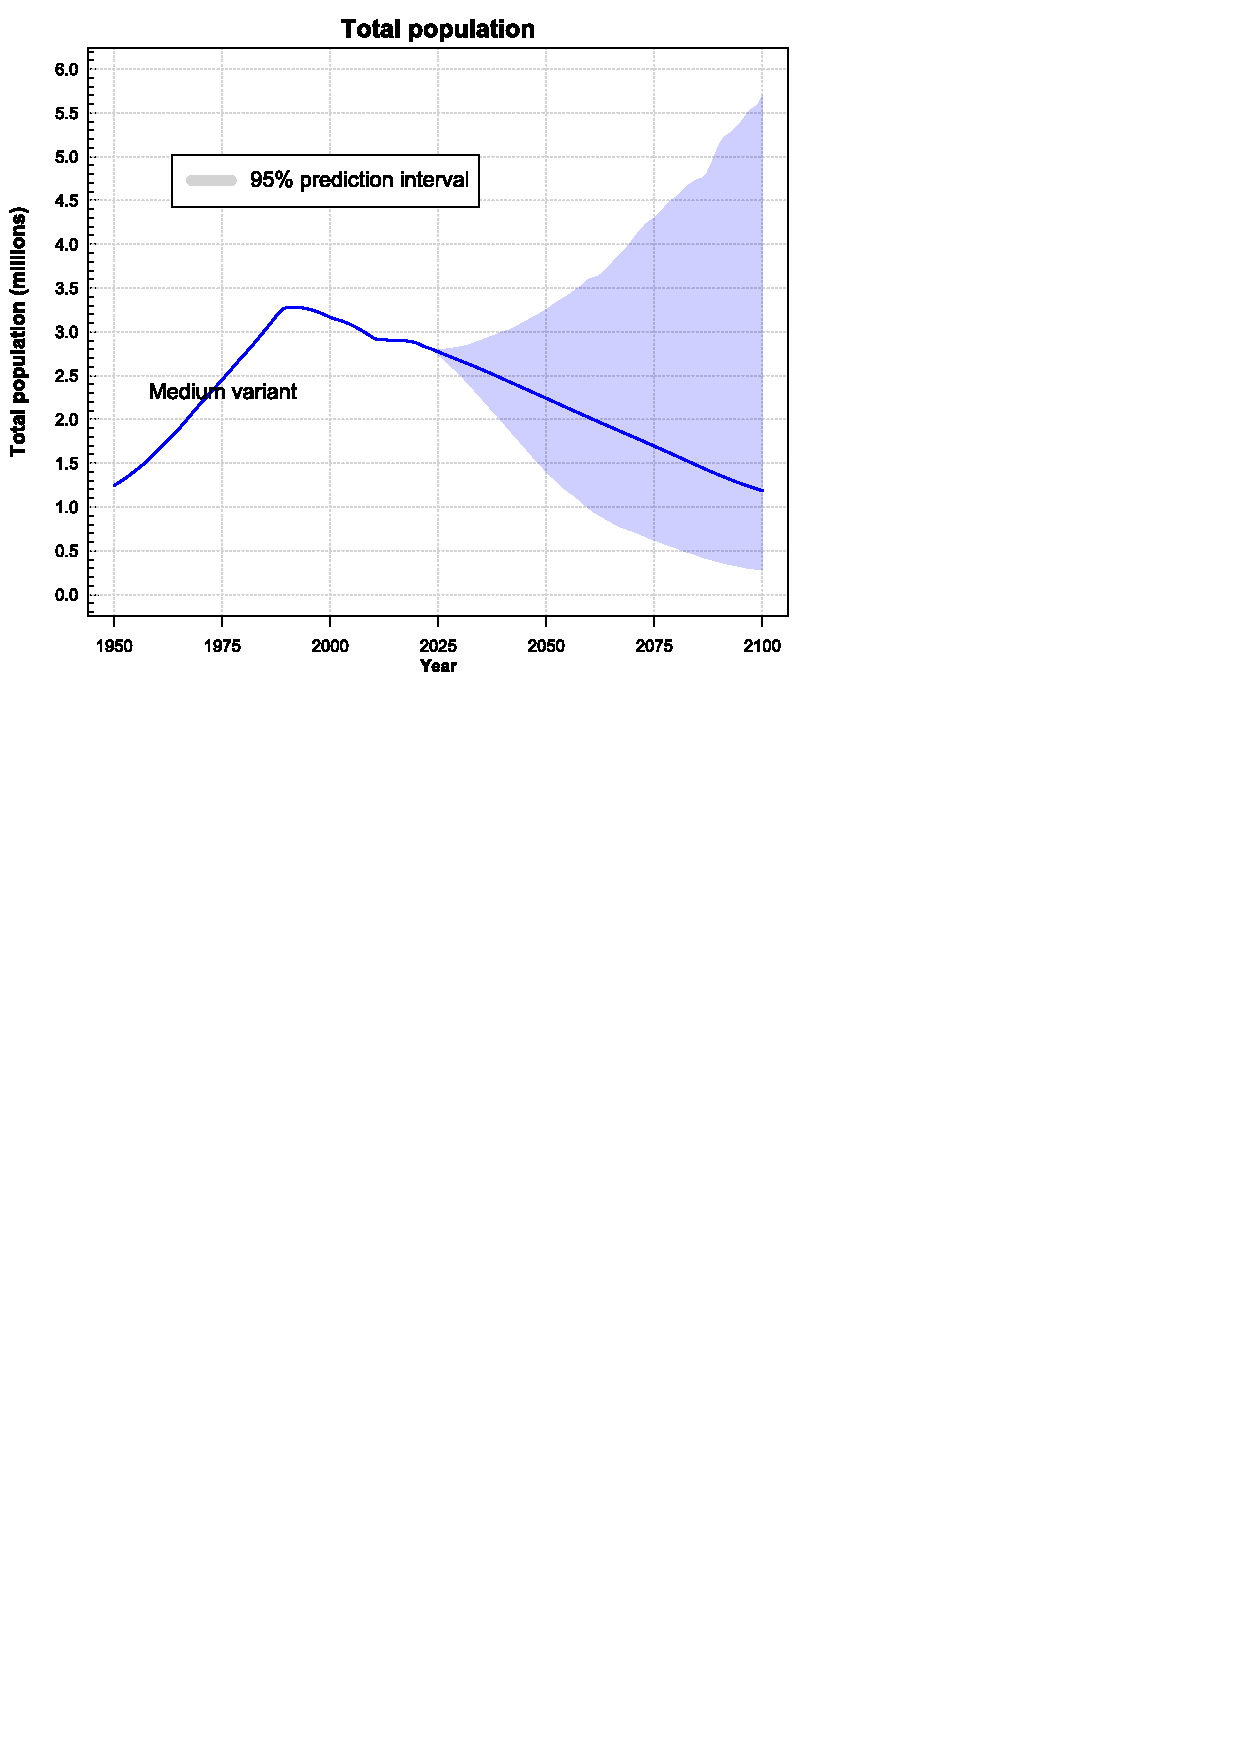
\includegraphics[width=\textwidth]{photos/1-Total population.html.pdf}
    \end{subfigure}
    \hfill
    \begin{subfigure}[b]{0.32\textwidth}
        \centering
        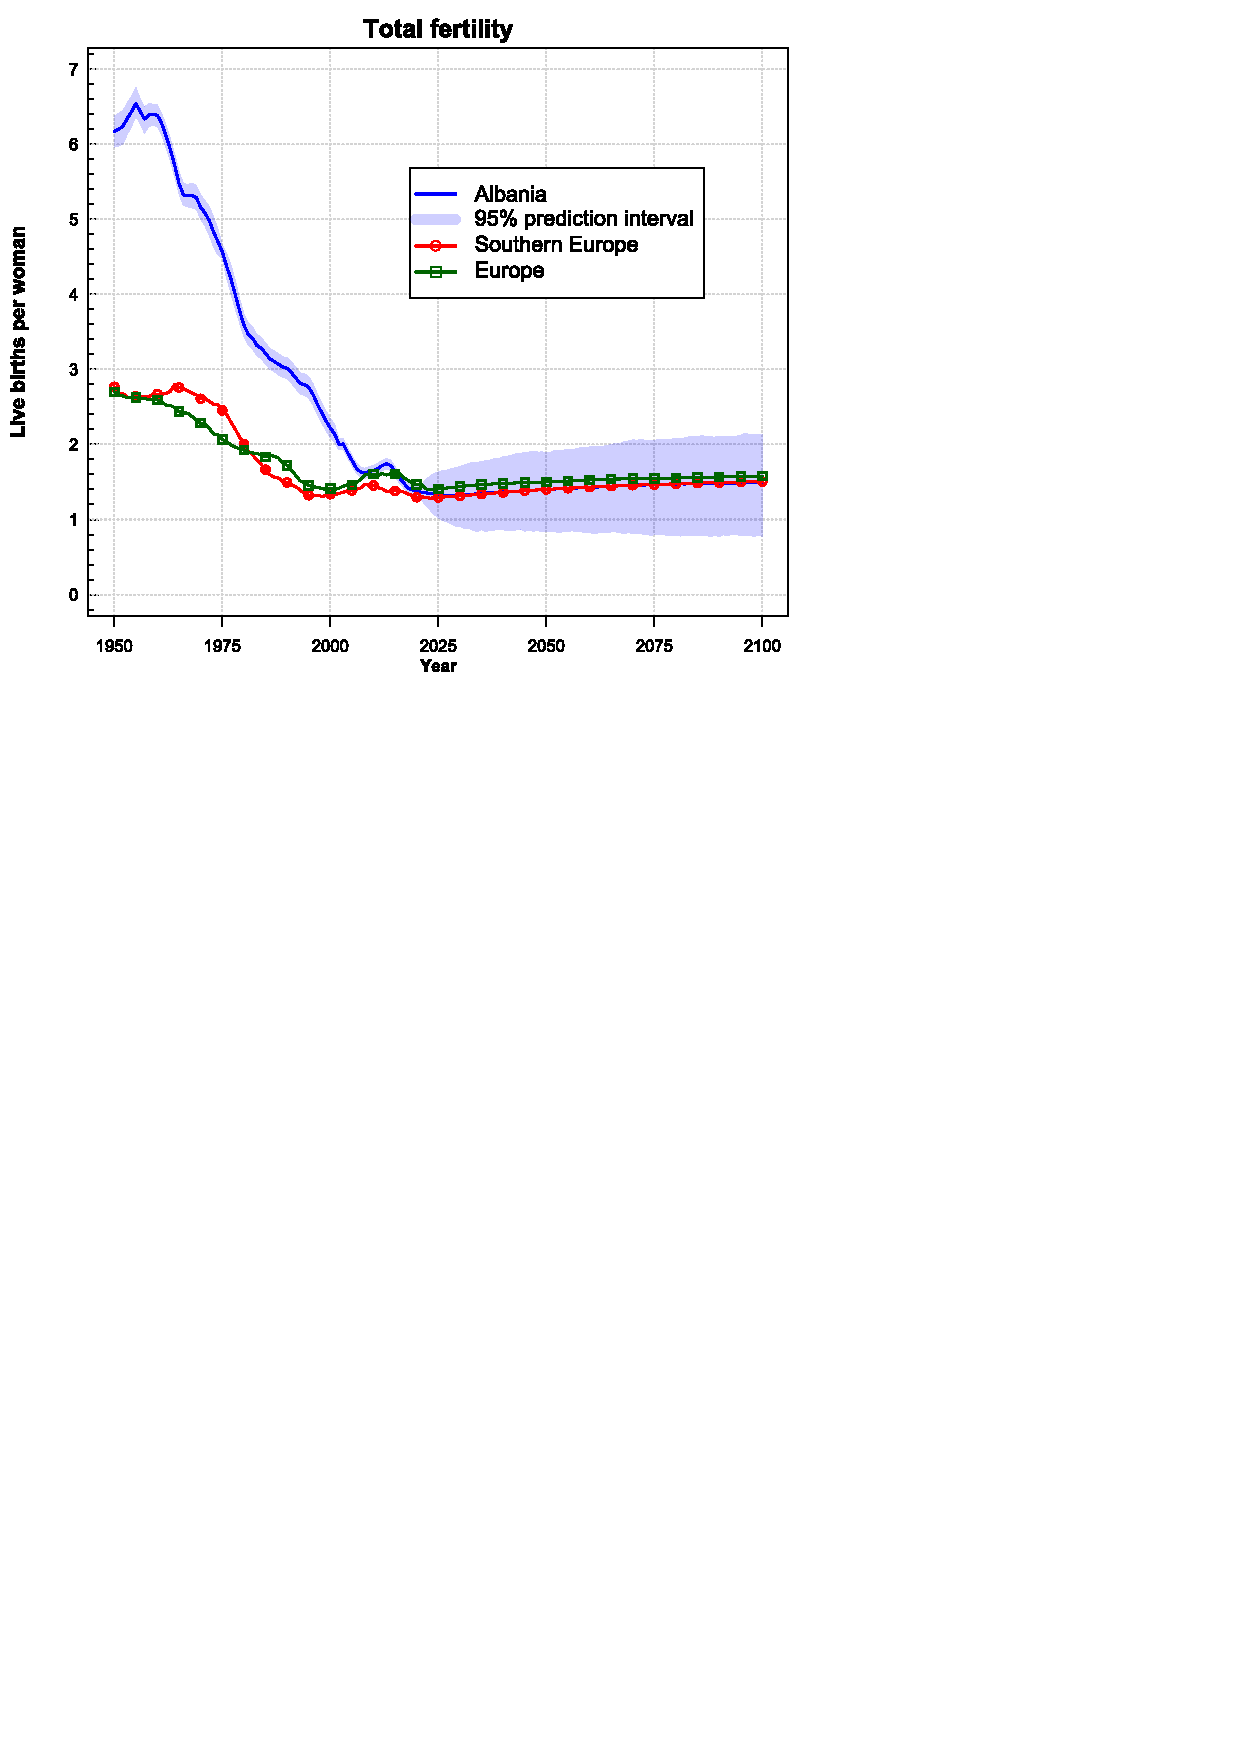
\includegraphics[width=\textwidth]{photos/6-Total fertility.html.pdf}
    \end{subfigure}
    \hfill
    \begin{subfigure}[b]{0.32\textwidth}
        \centering
        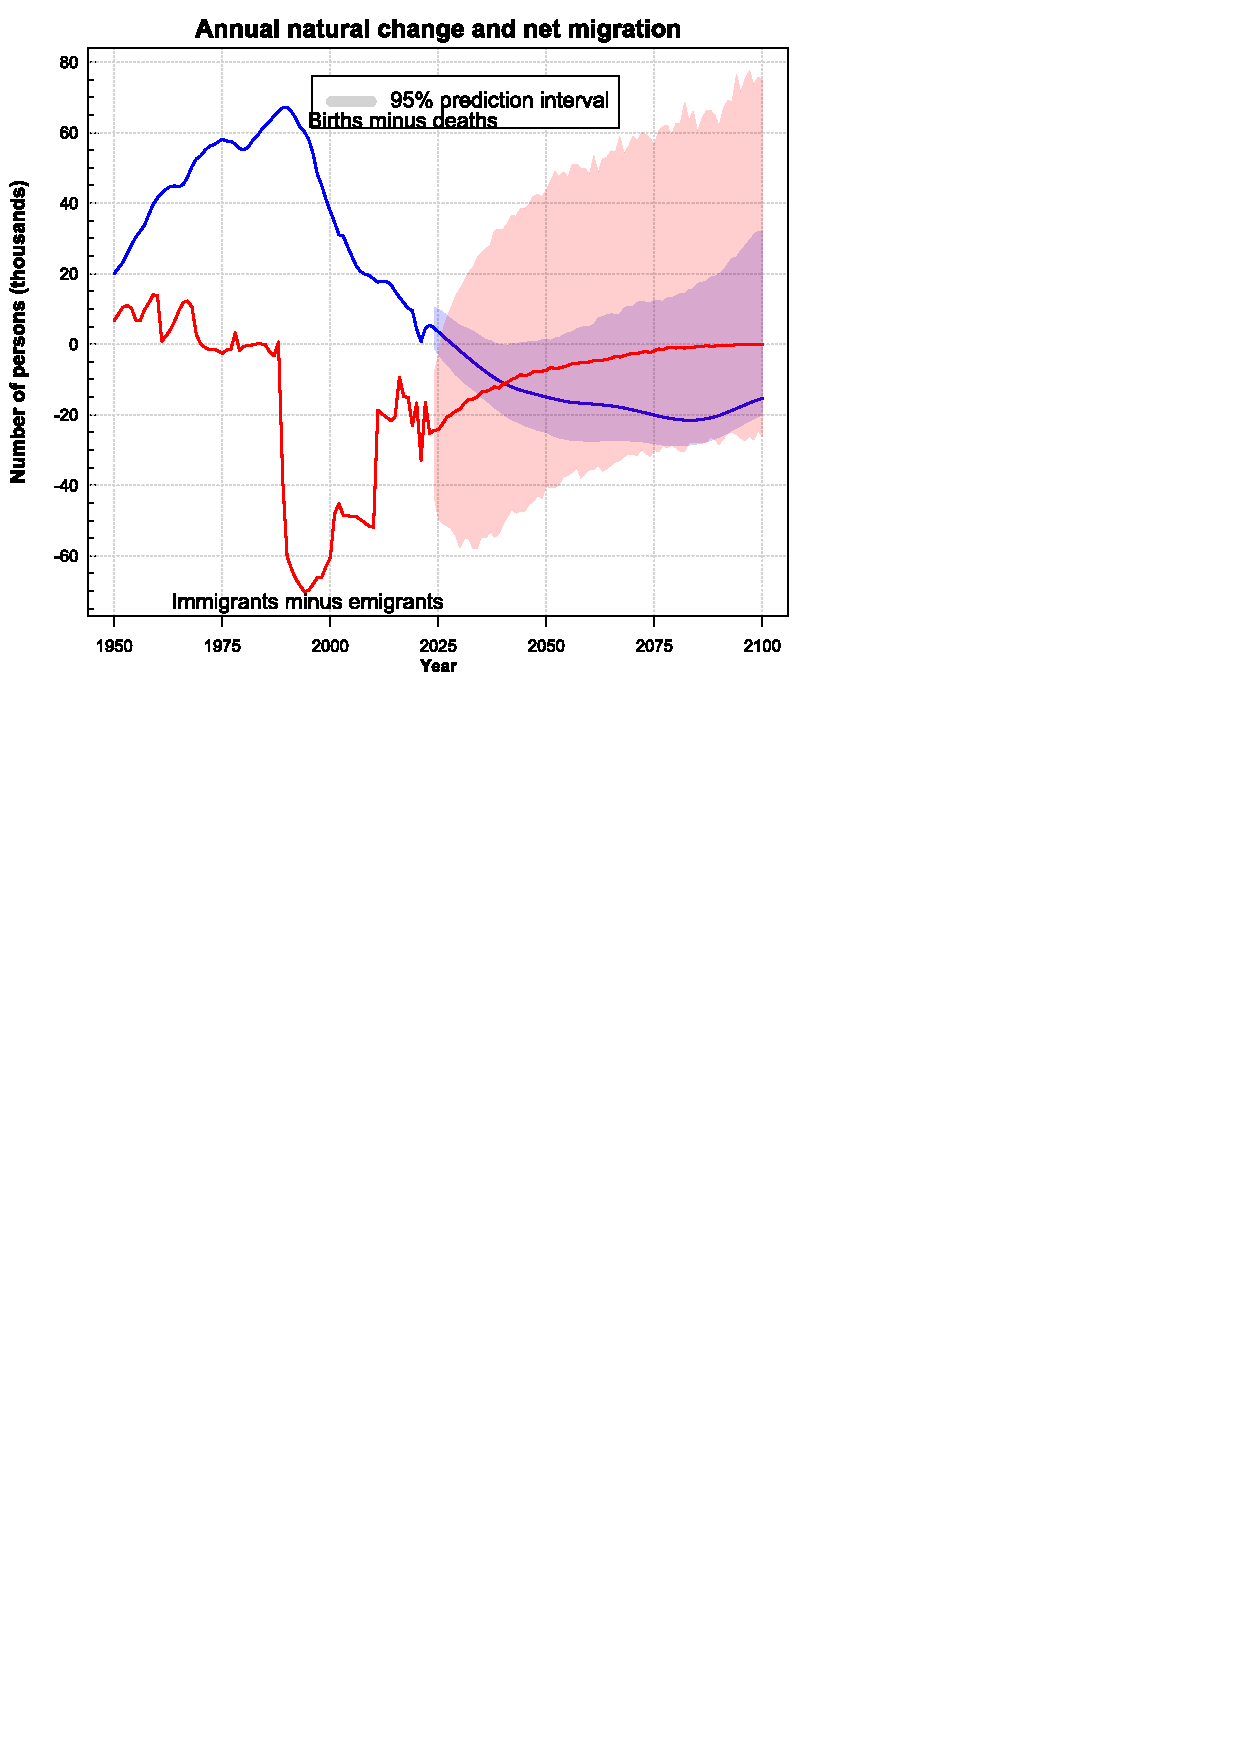
\includegraphics[width=\textwidth]{photos/10-Annual natural change and net migration.html.pdf}
    \end{subfigure}
    \caption{Graphs showing some demographic development of Albania \citep{unitednationsWorldPopulationProspects2024}}
    \label{fig:back-albaniaDemo}
\end{figure}
If it is to be granted entry into the \acrfull{eu} block, an ambition supported by its EU membership application in 2009 \citep{europeancouncilAlbaniaConsilium2025}, Albania will have to meet the demands of the EU Commission. The country will need to secure the production of renewable energy resources, such as solar power. The country also needs to increase development in rural areas, lacking institution building in these areas\citep{eucommissionAlbania2024Report2024}. Having only achieved full grid coverage for the first time in 2010 \citep{internationalrenewableenergyagencyTrackingSDG7Energy2023}, the rural population has been lagging behind the development in urban areas. Although  almost all energy production in Albania comes from hydroelectric plants, Albania tends to experience a power deficit. On average, between 2000 and 2022, they imported 20 percent of their electricity supply \citep{internationalenergyagencyAlbaniaCountriesRegions2025}. Albanian shares a power market with Kosovo, importing electricity from them through the Albanian Power Exchange\citep{albanianpowerexchangeHistoryALPEX2025}. Kosovo has 91\% of it's electricity generation from coal plants, making the imported energy from mostly fossil fuels\citep{internationalenergyagencyKosovoCountriesRegions2025}. 


\section{`Use the Sun' project background}
In 2024, Bright Products and Norsk Nødhjelp cooperated with The Door Albania to initiate the "Use the Sun" project. This project had the objectives Environmental Impact, Economic Benefits and Community Awareness - distributing \acrfull{shs} to various consumers, including private families, small companies and organizations, seeking to increase the production of clean energy and to educate communities about the benefit of solar power. More than 140 systems were delivered to participants. Most recipients were located in the northern part of Albania, near Shköder. Although different Bright models were distributed, all the systems belong to the same series from Bright Products and fall within the 30Wh to 80Wh range.

Norsk Nødhjelp has been present in Albania with humanitarian aid since 1996. Their work includes running a free daycare, delivering clothes, food and other equipment to people in need. Organizing social activities for children, youth and disabled people \citep{norsknodhjelpAlbania2025}. 

The motivation to do an evaluation of this project stems from the low amount of literature in the specific field. The research and literature on the subject of SHS are often contained to areas with no access to electricity, rather than where there is grid connection. For example This report from Rwanda \citep{asifGrameenShaktiExemplary2012} showing an exemplary case of the result of SHS in a rural off-grid area. Or this master thesis with a case study in Kenya \citep{gulbrandsenAssessingWhetherConnection2021}, making a detailed analysis about how SHS or microgrids can be implemented to increase access to electricity in a specific village.  


\section{Solar energy as a power source}
\label{ch:back:sec:solar}
\subsection{Lower costs of PV technology}
From 2010 to 2023, utility-scale \acrfull{pv} systems \acrfull{lcoe} fell from 0.460 USD per kWh, to 0.044 USD per kWh. Making PV technology's global weighted average LCOE 56\% lower than fossil fuel options 
 \citep{irena_renewable_2024}. PV system technology is expected to lower in LCOE even further. In figure \ref{fig:back-lcoe-nrl} NRL is expecting the price of residential PV to decrease substantially by 2050 \citep{nrlResidentialPV2024}. The costs decrease of PV systems help further the ambition of a green and fossil free energy mix. \citep{calvinIPCC2023Climate2023} refers to the decreased costs of solar allowing some regions to reduce their overall energy costs by replacing unsustainable energy sources with solar power. Also emphasizing that there needs to be a transition to renewable energy sources to reduce the emissions of greenhouse gasses. With the eminent future going towards an increase of \SI{1.5}{\celsius} above average within 2040, emissions needs to be reduced quickly \citep{calvinIPCC2023Climate2023}. 

\begin{figure}[H]
    \centering
    \begin{subfigure}[b]{0.48\textwidth}
        \centering
        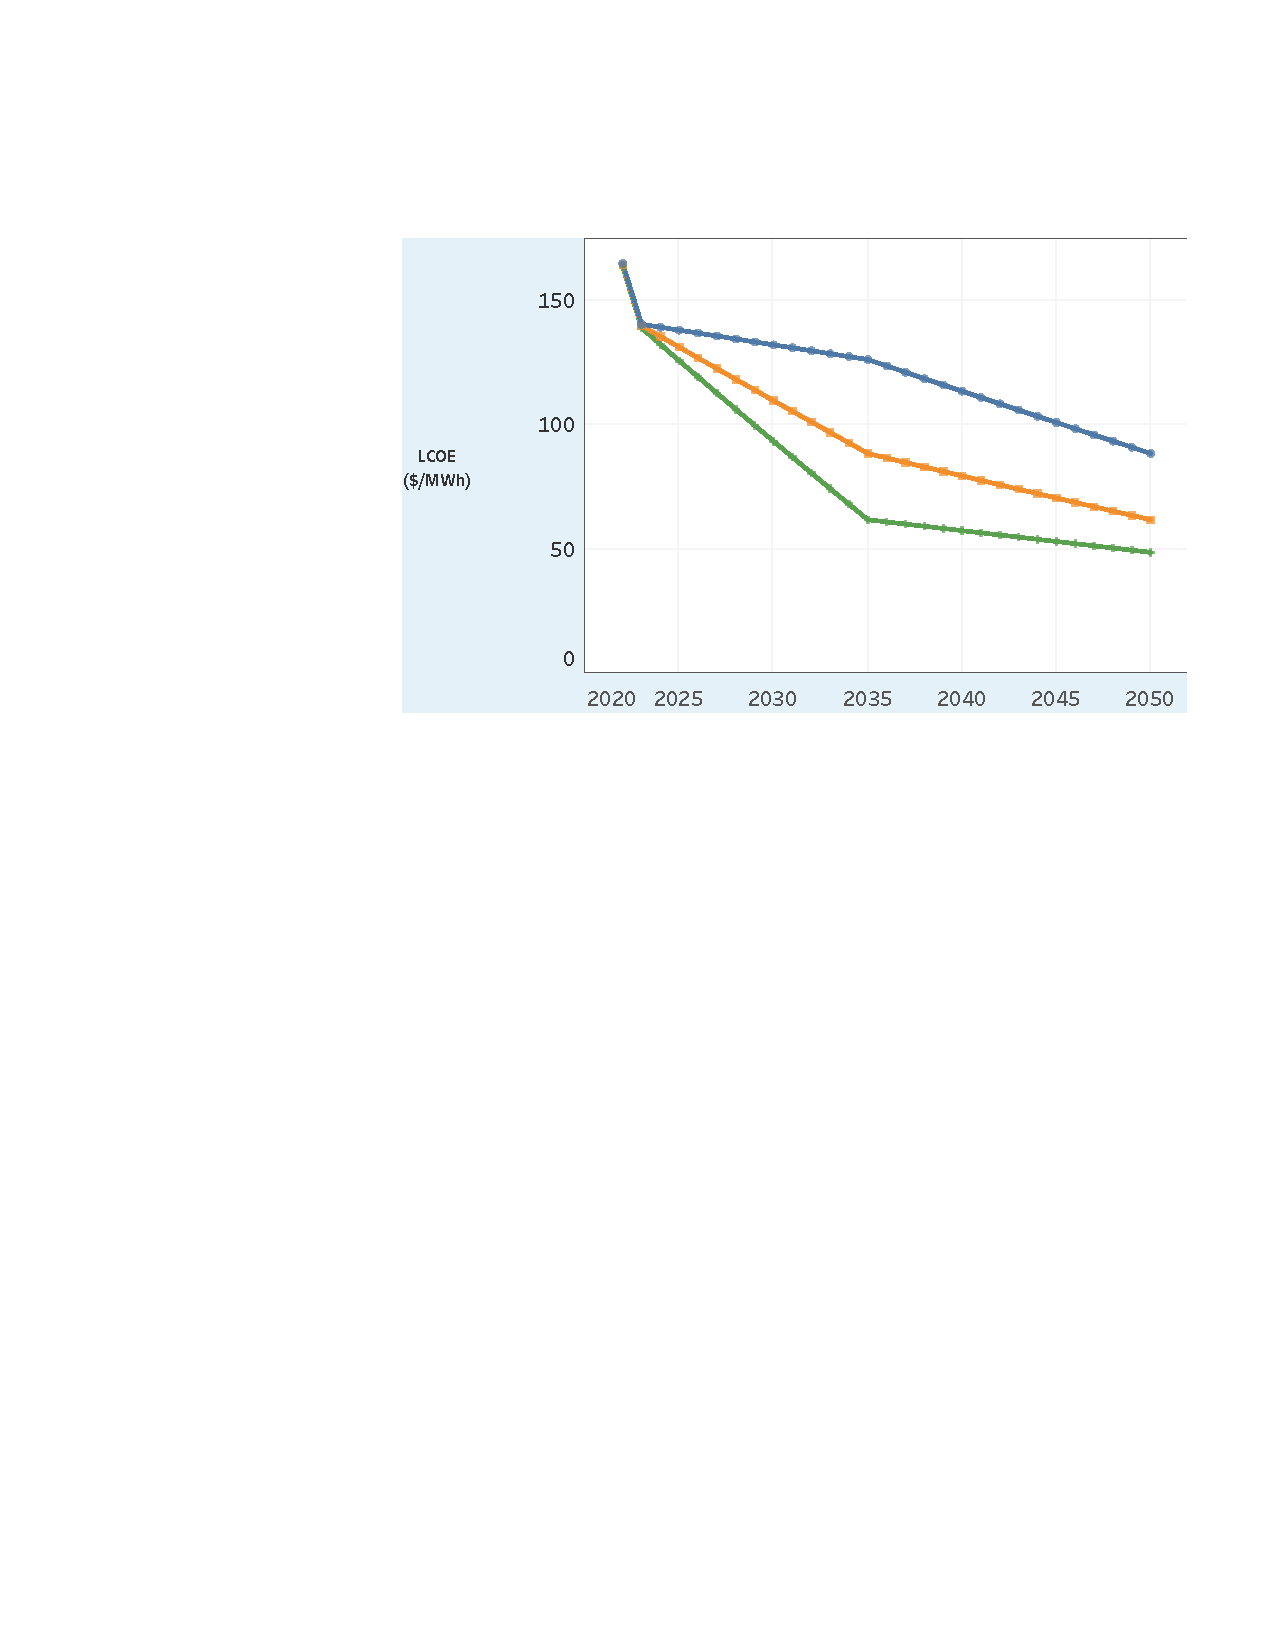
\includegraphics[width=\textwidth]{photos/LCOE_ResidentialPV_NRL.pdf}
        \caption{NRL prediction for residential PV systems. Using scenario of average 4,5 to \SI{5}{\kilo\watt\hour\per\square\meter\per\day}. The three scenarios are conservative (blue), moderate (orange) and advanced (green).}
    \end{subfigure}
    \hfill
    \begin{subfigure}[b]{0.48\textwidth}
        \centering
        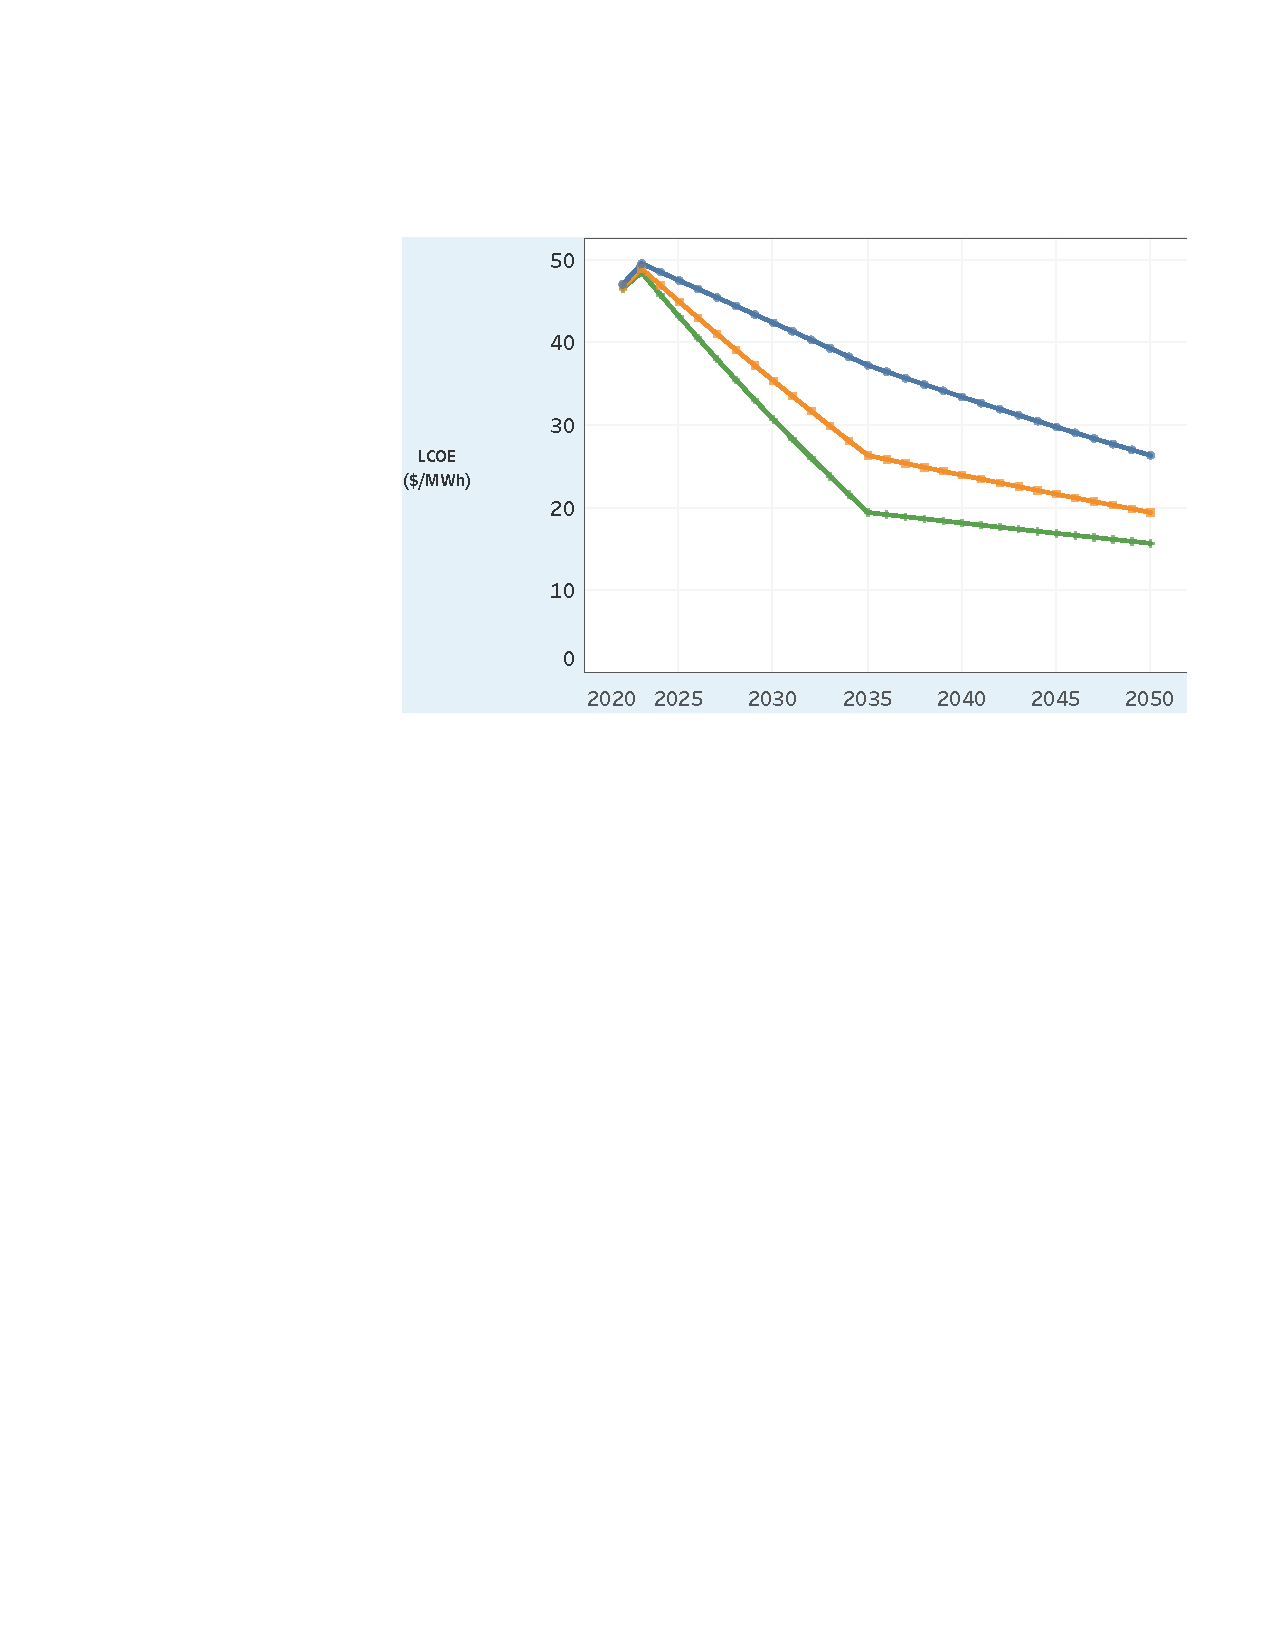
\includegraphics[width=\textwidth]{photos/LCOE_UtilityPV_NRL.pdf}
        \caption{NRL prediction for utility PV systems. Using scenario of average 4,5 to \SI{5}{\kilo\watt\hour\per\square\meter\per\day}. The three scenarios are conservative (blue), moderate (orange) and advanced (green).}
    \end{subfigure}
    \caption{}
    \label{fig:back-lcoe-nrl}
\end{figure}

\subsection{Solar energy in Albania}
Solar energy accounted for 2.3\% of electricity production in Albania in 2022\citep{internationalenergyagencyAlbaniaCountriesRegions2025}. Green Energy News Balkan posted an article claiming it is now 6\%, and that there is plans to further increase the capacity by  235MW \citep{igortodorovicSolarPowerDevelopers2025}. In January 2025, Albania, Italy and United Arab Emirates signed a three-way energy cooperation deal. It's purpose was to increase Albanian's solar and wind production, and to export power to Italy via underwater cables\citep{euronewsgreenItalyAlbaniaAgree2025}. These news show that Albania seeks to expand their capacity within solar energy. 

A 2021 report by International Renewable Energy Agency states that Albania's technical potential for the deployment of solar PV is estimated at 2378 MWh. Also purposing a plan for 2030 of an installed capacity of 1697 MWh\citep{irena_renewables_2021}. The report also talks about the importance of raising public awareness to the adoption of the technology. Figure \ref{fig:back-albaniacapacitymap} shows the areas that the report suggested for installing PV systems. The areas suggested mostly occur close to the coast, where the land is flat. Skhöder, the area most relevant for the project, is marked as a suggested spot. 

\begin{figure}[H]
    \centering
    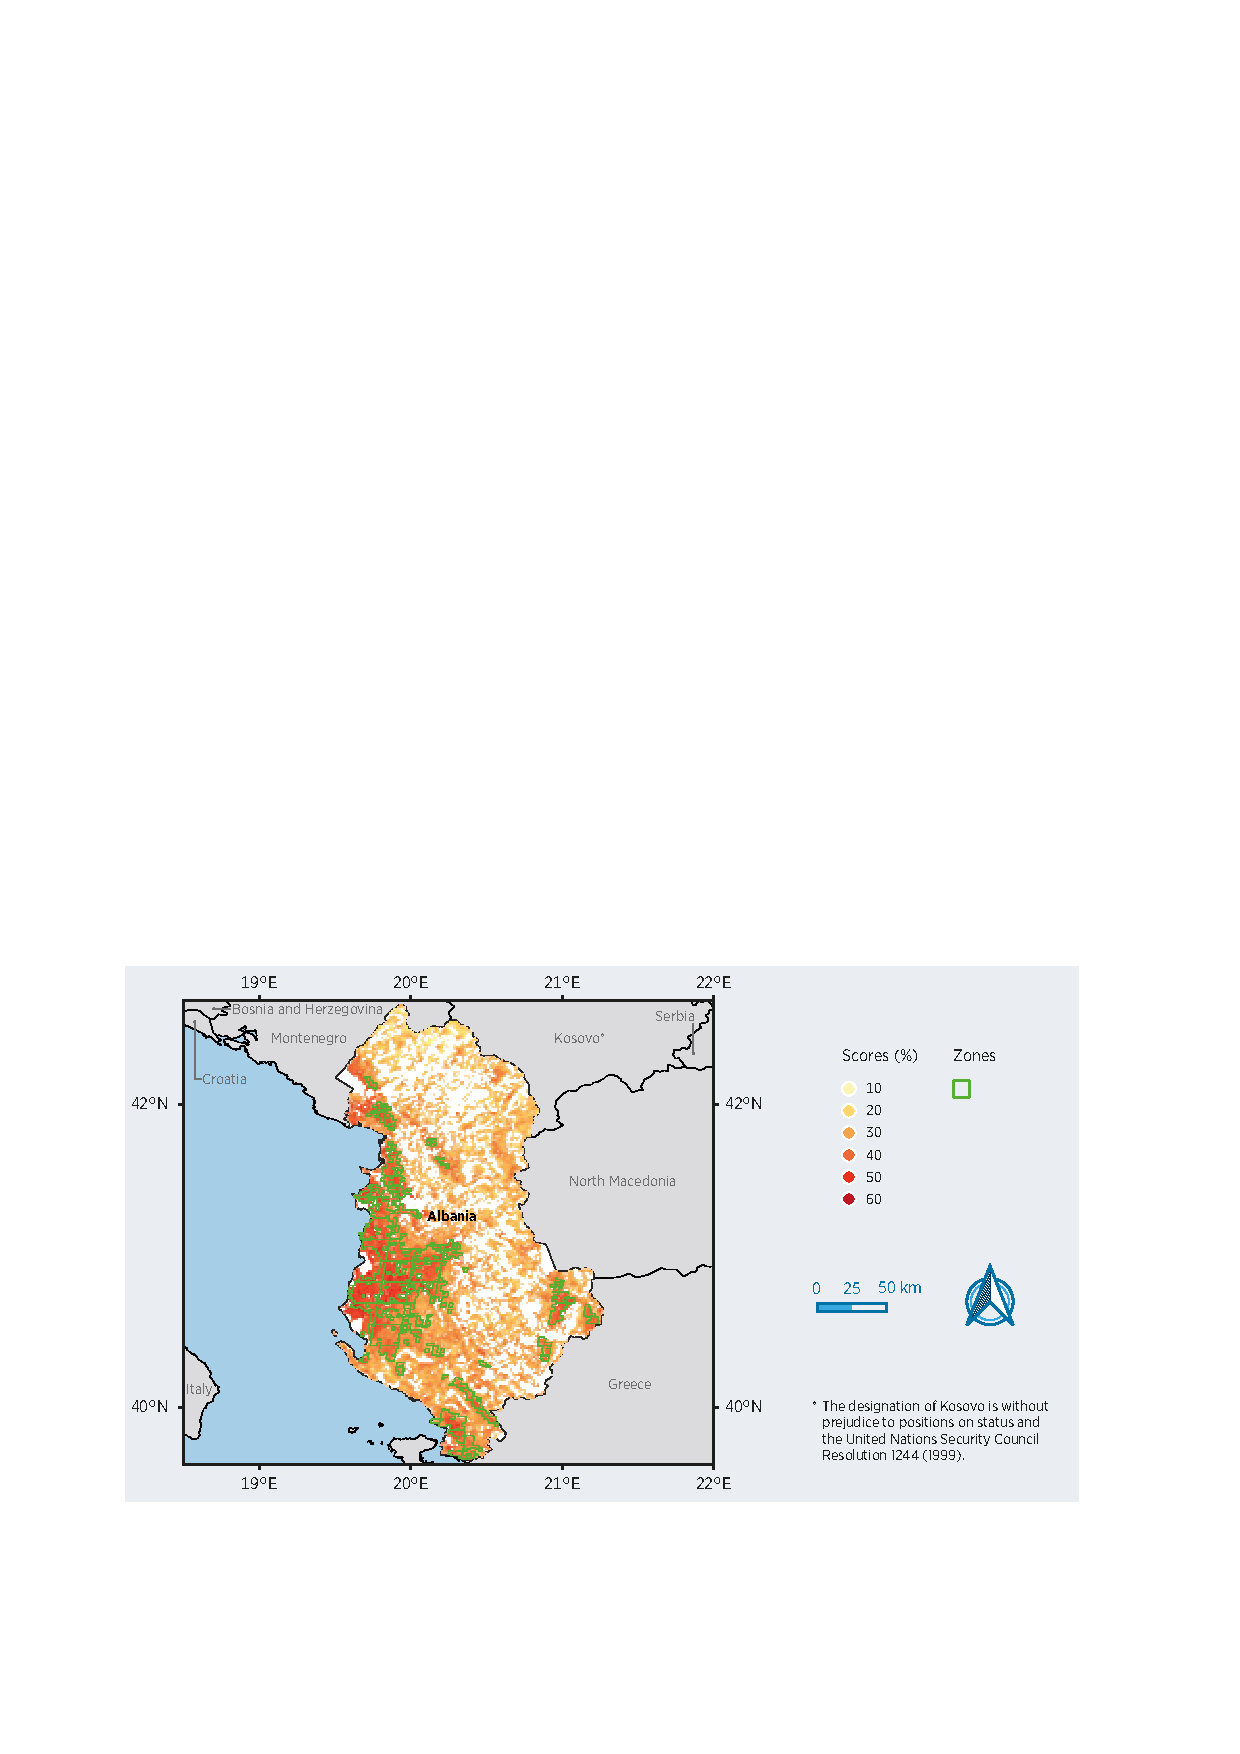
\includegraphics[width=\linewidth]{photos/Albania_solarPVCapacity_map.pdf}
    \caption{Suitable areas for solar PV development and zones with highest potential \citep{irena_renewables_2021}.}
    \label{fig:back-albaniacapacitymap}
\end{figure}

\subsection{SHS as a power source}
\acrfull{shs} have been used for decades to provide renewable solar energy to areas without access to electricity. Consisting of a simple design with a solar panel, battery and lighting - SHS is a robust and easy product to use. Making use of solar power these products are often introduced in areas with high irradiance, such as Sub-Saharan Africa. Introducing SHS to developing countries has been shown to introduce problems. Access to skilled technicians and general knowledge about the product has been highlighted as a reoccurring problem \citep{chaureyAssessmentEvaluationPV2010}. The high initial cost of purchasing a SHS is another one of the main causes hindering adoption of the technology, sometimes reaching up to half of the user's income. Product quality, maintenance and user training have also been shown to be barriers to entry\citep{girardeauHouseholdSolarAdoption2018}. 


\section{Existing Approaches/Baselines}
Since there are a lot of different cases for SHS, there are also a lot of different approaches analyzing a SHS project. Most studies look at the \acrfull{lcoe}, and in general, look at either the technical design of the systems or economical viability of the systems. These fiscal measures serve as a solid baseline for a project's success, but often do not tell the entire story. \citep{thomasPESTLEAnalysisSolar2021a} did a \acrshort{pestel} analysis for a broader evaluation of the subject. Though the format offers a wider result, they found a lack data in their legal and environmental section of the analysis. This is caused by the limited amount of available research and information to evaluate this. 

One study proposes a new way of analyzing the success of SHS projects\citep{holtorfModelEvaluateSuccess2015}. It evaluates based on self set goals for each project and the different stakeholders in the project. Each self set goal is then ranked by  importance and degree of achievement, giving it a score based on the stakeholders subjective experience. 

\citep{lervikTechnoEconomicAnalysisRural2021} use simulation and load profiles to create an estimated value for the panels and their effect. This approach offers a solid foundation for the production capabilities of the equipment. 

SHS typically does not store data about product usage such as battery charge cycles and electricity usage. Recording and storing data would increase cost, and demand some power to maintain the circuit. \citep{lopez-vargasIoTApplicationRealTime2019} have created a logging feature that communicates with 3G to send data as consumption, production, battery state and weather data. Although their solution is low cost compared to commercial alternatives, the conclusion is that this is costly on small-scale systems.

To account for a lack of data tracking from the equipment, \citep{mannesEnduserEvaluationSolar2017} used a load profile based on detailed interview questions.  
Data are gathered on when the power was used, and how much it was used within a day. Using these data \citep{mannesEnduserEvaluationSolar2017} can also compare the daily load against the theoretical charge given in various days, to see how the production and consumption match.



One way to gather data is through qualitative research. Interviews with consumers about their experiences are used in several SHS studies e.g., \citep{mannesEnduserEvaluationSolar2017},\citep{asifGrameenShaktiExemplary2012}, \citep{beyeneSocioeconomicImpactsSolar2024}. On the one hand, semi-structured interviews provide a good baseline, offering the possibility to ask additional questions outside of the structured questions. On the other hand, structured questions give the possibility to easily compare results and organize the data.

Sub-Saharan Africa is often used as study area in the literature. \citep{kizilcecSolarHomeSystems2020} shows that the most common topics for SHS in Sub-Saharan Africa are the business aspects and the design of the systems. More research around the institutional barriers, and the regulatory framework is called for \citep{kizilcecSolarHomeSystems2020}.





